% Gabarit pandoc des corrigés publiés (brut et guidé). Contenu sans marque ni nom de site.
% Compilation : lualatex (latexmk -lualatex).
% Le Markdown reste la source unique : ne pas éditer ce fichier .tex à la main.
\documentclass[11pt,a4paper]{article}

% --- Moteur, polices (Latin Modern) et langue ---------------------------------
\usepackage{iftex}
\ifLuaTeX\else\errmessage{Ce document se compile avec lualatex}\fi
\usepackage{amsmath,amssymb,mathtools}
\usepackage{fontspec}
% mathrm=sym : \mathrm prend ses glyphes dans la police mathématique (ℓ, μ, Ω), comme KaTeX.
\usepackage[math-style=TeX,bold-style=TeX,mathrm=sym]{unicode-math}
% Repli pour les glyphes absents de Latin Modern (indices et exposants Unicode,
% flèches, filets des schémas en texte, symboles) : DejaVu, puis Latin Modern Math
% (ℓ, lettres mathématiques Unicode des légendes).
\directlua{
  luaotfload.add_fallback("repliTexte", {"DejaVuSerif:mode=harf;", "DejaVuSans:mode=harf;", "file:latinmodern-math.otf:mode=harf;"})
  luaotfload.add_fallback("repliMono", {"DejaVuSansMono:mode=harf;", "DejaVuSans:mode=harf;", "file:latinmodern-math.otf:mode=harf;"})
}
\setmainfont{Latin Modern Roman}[RawFeature={fallback=repliTexte}]
\setsansfont{Latin Modern Sans}[RawFeature={fallback=repliTexte}]
\setmonofont{Latin Modern Mono}[RawFeature={fallback=repliMono}]
\setmathfont{Latin Modern Math}
\usepackage[french]{babel}
\frenchsetup{SmallCapsFigTabCaptions=false}

% --- Mise en page --------------------------------------------------------------
\usepackage[a4paper,margin=2.2cm,headheight=14pt,footskip=1.2cm]{geometry}
\usepackage{microtype}
\setlength{\emergencystretch}{4em}
\tolerance=1500
\setlength{\parindent}{0pt}
\setlength{\parskip}{0.55\baselineskip plus 2pt minus 1pt}
\usepackage{xcolor}
% Gris nommés : babel-french rend « ! » actif dans le document.
\definecolor{gris2}{gray}{0.98}
\definecolor{gris3}{gray}{0.97}
\definecolor{gris5}{gray}{0.95}
\definecolor{gris35}{gray}{0.65}
\definecolor{gris40}{gray}{0.60}
\definecolor{gris45}{gray}{0.55}
\definecolor{gris50}{gray}{0.50}
\definecolor{gris55}{gray}{0.45}
\definecolor{gris60}{gray}{0.40}
\definecolor{gris65}{gray}{0.35}
\definecolor{gris70}{gray}{0.30}
\definecolor{gris80}{gray}{0.20}
\definecolor{gris85}{gray}{0.15}
\usepackage{graphicx}
\usepackage{float}
\usepackage{caption}
\captionsetup{font=small,labelformat=empty,justification=centering}
\usepackage{booktabs,longtable,array,multirow,calc}
\usepackage{siunitx}
\sisetup{locale=FR}
\usepackage[version=4]{mhchem}
\usepackage{listings}
\usepackage{fancyhdr}
\usepackage{lastpage}
\usepackage[most]{tcolorbox}
\usepackage{enumitem}
\setlist{nosep,leftmargin=*,topsep=2pt}
\usepackage[hidelinks,unicode]{hyperref}
\usepackage{bookmark}
\hypersetup{pdftitle={CCINP TPC — Informatique 2026},pdfauthor={Rédigé par IA},pdfcreator={LaTeX},pdfsubject={Corrigé brut}}
\usepackage{xurl}

% --- Pandoc : listes, tableaux, figures ----------------------------------------
\providecommand{\passthrough}[1]{#1}
\providecommand{\tightlist}{\setlength{\itemsep}{0pt}\setlength{\parskip}{0pt}}

\makeatletter
\def\maxwidth{\ifdim\Gin@nat@width>\linewidth\linewidth\else\Gin@nat@width\fi}
\def\maxheight{\ifdim\Gin@nat@height>0.55\textheight 0.55\textheight\else\Gin@nat@height\fi}
\makeatother
\setkeys{Gin}{width=\maxwidth,height=\maxheight,keepaspectratio}
\setcounter{secnumdepth}{-\maxdimen}
\providecommand{\pandocbounded}[1]{#1}

% --- Code (listings) -----------------------------------------------------------
\lstset{
  basicstyle=\ttfamily\small,
  columns=fullflexible,
  keepspaces=true,
  breaklines=true,
  breakatwhitespace=false,
  postbreak=\mbox{\textcolor{gris50}{$\hookrightarrow$}\space},
  frame=single,
  rulecolor=\color{gris35},
  framesep=4pt,
  xleftmargin=5pt,xrightmargin=5pt,
  backgroundcolor=\color{gris3},
  keywordstyle=\bfseries,
  commentstyle=\color{gris65},
  stringstyle=\color{gris80},
  showstringspaces=false,
  tabsize=4,
  extendedchars=true,
  aboveskip=6pt,belowskip=6pt,
}

% --- Macros des corrigés (KaTeX ↔ LaTeX) ---------------------------------------
% Les corrigés sont écrits pour KaTeX : on définit ici ce que KaTeX connaît et
% que LaTeX n'a pas, sans jamais retoucher le Markdown.
\providecommand{\R}{\mathbb{R}}
\providecommand{\N}{\mathbb{N}}
\providecommand{\Z}{\mathbb{Z}}
\providecommand{\Q}{\mathbb{Q}}
\providecommand{\C}{\mathbb{C}}
\providecommand{\dd}{\mathrm{d}}
\providecommand{\llbracket}{\lBrack}
\providecommand{\rrbracket}{\rBrack}
\providecommand{\lBrace}{\lbrace}
\providecommand{\rBrace}{\rbrace}
\providecommand{\Box}{\square}
\providecommand{\Diamond}{\lozenge}
\providecommand{\varnothing}{\emptyset}
\providecommand{\argmax}{\operatorname*{arg\,max}}
\providecommand{\argmin}{\operatorname*{arg\,min}}
\renewcommand{\leq}{\leqslant}
\renewcommand{\geq}{\geqslant}

% Équation hors texte : réduite à la largeur de la ligne si elle déborde.
\newsavebox{\boiteequation}
\newcommand{\equationajustee}[1]{%
  \sbox{\boiteequation}{$\displaystyle #1$}%
  \ifdim\wd\boiteequation>\linewidth
    \[\resizebox{\linewidth}{!}{\usebox{\boiteequation}}\]%
  \else
    \[#1\]%
  \fi}

% --- Encadrés pédagogiques (sobres, lisibles en noir et blanc) -----------------
\tcbset{
  encadre/.style={
    enhanced,breakable,sharp corners,
    colback=white,colframe=gris55,
    boxrule=0.4pt,leftrule=2.2pt,
    left=6pt,right=6pt,top=3pt,bottom=3pt,
    before skip=6pt,after skip=6pt,
    fonttitle=\bfseries\small,coltitle=black,
    attach title to upper,after title={\quad},
    parbox=false,
  }
}
\newtcolorbox{indication}[1]{encadre,colframe=gris45,colback=gris2,title={Indication~#1}}
\newtcolorbox{methode}{encadre,colframe=gris70,title={Méthode}}
\newtcolorbox{piege}{encadre,colframe=gris85,boxrule=0.8pt,leftrule=2.2pt,title={Piège}}
\newtcolorbox{jury}{encadre,colframe=gris60,colback=gris5,title={Jury}}
\newtcolorbox{encadrenote}{encadre,colframe=gris40}

% --- Titres de section ---------------------------------------------------------
\usepackage{titlesec}
\titleformat{\section}{\Large\bfseries}{}{0pt}{}
\titleformat{\subsection}{\large\bfseries}{}{0pt}{}
\titleformat{\subsubsection}{\normalsize\bfseries}{}{0pt}{}
\titlespacing*{\section}{0pt}{14pt plus 4pt minus 2pt}{6pt}
\titlespacing*{\subsection}{0pt}{10pt plus 3pt minus 2pt}{4pt}
\titlespacing*{\subsubsection}{0pt}{8pt plus 2pt minus 2pt}{2pt}

% --- En-tête et pied de page ---------------------------------------------------
\pagestyle{fancy}
\fancyhf{}
\fancyhead[L]{\small\textsc{Corrigé brut} · CCINP TPC}
\fancyhead[R]{\small Informatique 2026}
\fancyfoot[L]{\footnotesize Corrigé rédigé par IA, non officiel}
\fancyfoot[R]{\footnotesize \thepage\,/\,\pageref*{LastPage}}
\renewcommand{\headrulewidth}{0.4pt}
\renewcommand{\footrulewidth}{0pt}
\fancypagestyle{plain}{\fancyhf{}\fancyfoot[R]{\footnotesize \thepage\,/\,\pageref*{LastPage}}\fancyfoot[L]{\footnotesize Corrigé rédigé par IA, non officiel}\renewcommand{\headrulewidth}{0pt}}

\begin{document}
\thispagestyle{plain}
\begin{center}
  {\small\scshape Corrigé brut}\par\smallskip
  {\LARGE\bfseries CCINP TPC — Informatique 2026\par}\medskip
  {\large CCINP · TPC · Informatique · 2026\par}
\end{center}
\vspace{2pt}\hrule\vspace{8pt}

\emph{Corrigé rédigé par IA, non officiel. Signalez toute erreur.}

Épreuve TPC5IN, 3 heures, calculatrice interdite. Code en Python (Partie I) et en SQL (Partie II). Les questions Q2, Q5, Q12, Q16, Q22 et Q23 se rédigent dans les cadres du Document Réponse (DR) ; les squelettes du DR sont reproduits et complétés ci-dessous.

Notations : la case de la ligne \(i\) et de la colonne \(j\) est notée \((i, j)\). Lignes et colonnes sont numérotées à partir de \(0\), les lignes de haut en bas et les colonnes de gauche à droite.

\hypertarget{partie-i-des-algorithmes-pour-ruxe9soudre-le-probluxe8me-des-n-reines}{%
\section{Partie I --- Des algorithmes pour résoudre le problème des n reines}\label{partie-i-des-algorithmes-pour-ruxe9soudre-le-probluxe8me-des-n-reines}}

\hypertarget{i.1-introduction}{%
\subsection{I.1 --- Introduction}\label{i.1-introduction}}

\hypertarget{q1}{%
\subsubsection{Q1}\label{q1}}

Dans la configuration perdante de la figure 4, les reines occupent les cases \((0,0),\ (1,2),\ (2,3),\ (3,1)\).

Il y a une reine par ligne et les colonnes \(0, 2, 3, 1\) sont distinctes.

Mais les reines \((1,2)\) et \((2,3)\) ont le même écart de lignes et de colonnes :

\equationajustee{\begin{aligned}
2 - 1 &= 1 \quad \text{(lignes)} \\
3 - 2 &= 1 \quad \text{(colonnes)}
\end{aligned}}

Elles sont donc sur la même diagonale descendante (et adjacentes) : la reine de la ligne 1 contrôle la case de la reine de la ligne 2. \textbf{La configuration perdante place deux reines sur une même diagonale descendante : elle ne respecte pas la consigne.}

\hypertarget{q2}{%
\subsubsection{Q2}\label{q2}}

On lit chaque ligne de haut en bas et on note la colonne de sa reine :

\equationajustee{\boxed{\begin{aligned}{}&\text{gagnante : } L = [2, 0, 3, 1] \\
&\text{perdante : } L = [0, 2, 3, 1]
\end{aligned}}}

Contrôle : pour la perdante, les \(L[i] - i\) valent \(0, 1, 1, -2\) ; la valeur \(1\) répétée retrouve le conflit de Q1.

\hypertarget{i.2-mise-en-place-dun-affichage}{%
\subsection{I.2 --- Mise en place d'un affichage}\label{i.2-mise-en-place-dun-affichage}}

\hypertarget{q3}{%
\subsubsection{Q3}\label{q3}}

\begin{lstlisting}[language=Python]
def ligne(n):
    """Renvoie une liste de n zéros."""
    return [0] * n
\end{lstlisting}

\texttt{ligne(5)} renvoie \texttt{{[}0,\ 0,\ 0,\ 0,\ 0{]}} (et \texttt{ligne(0)} renvoie \texttt{{[}{]}}).

\hypertarget{q4}{%
\subsubsection{Q4}\label{q4}}

Chaque appel à \texttt{ligne(n)} crée une liste neuve, donc les \(n\) sous-listes sont distinctes en mémoire. L'écriture \texttt{{[}{[}0{]}\ *\ n{]}\ *\ n} est exclue : elle répète \(n\) fois \textbf{la même} liste, et modifier \texttt{G{[}0{]}{[}0{]}} modifierait toutes les lignes.

\begin{lstlisting}[language=Python]
def grille(n):
    """Renvoie n listes distinctes contenant chacune n zéros."""
    G = []
    for i in range(n):
        G.append(ligne(n))   # nouvelle liste à chaque tour
    return G
\end{lstlisting}

\hypertarget{q5}{%
\subsubsection{Q5}\label{q5}}

Squelette du DR complété : on écrit directement le \(1\) à sa place, sans parcourir toutes les cases.

\begin{lstlisting}[language=Python]
def remplir(L):
    # On récupère la taille de L
    n = len(L)
    # On crée la liste de listes G
    G = grille(n)
    # On remplit G à l'aide de L
    for i in range(n):
        G[i][L[i]] = 1      # la reine de la ligne i est en colonne L[i]
    return G
\end{lstlisting}

La boucle de remplissage fait \texttt{len(L)} tours de coût constant : elle est en \(O(\texttt{len(L)})\), contre \(O(n^2)\) pour une double boucle testant \texttt{L{[}i{]}\ ==\ j}.

(La création de la grille par \texttt{grille(n)} reste en \(O(n^2)\), puisqu'il y a \(n^2\) cases à créer.) \texttt{remplir(\allowbreak{}{[}1,\allowbreak{}\ 3,\allowbreak{}\ 0,\allowbreak{}\ 2{]}\allowbreak{})\allowbreak{}} renvoie bien \texttt{{[}{[}0,\allowbreak{}\ 1,\allowbreak{}\ 0,\allowbreak{}\ 0{]}\allowbreak{},\allowbreak{}\ {[}0,\allowbreak{}\ 0,\allowbreak{}\ 0,\allowbreak{}\ 1{]}\allowbreak{},\allowbreak{}\ {[}1,\allowbreak{}\ 0,\allowbreak{}\ 0,\allowbreak{}\ 0{]}\allowbreak{},\allowbreak{}\ {[}0,\allowbreak{}\ 0,\allowbreak{}\ 1,\allowbreak{}\ 0{]}\allowbreak{}{]}\allowbreak{}}.

\hypertarget{q6}{%
\subsubsection{Q6}\label{q6}}

\begin{lstlisting}[language=Python]
def affiche(G):
    """Affiche la grille G ligne par ligne ; ne renvoie rien."""
    for rangee in G:
        print(rangee)
\end{lstlisting}

La variable de boucle n'est pas appelée \texttt{ligne}, pour ne pas masquer la fonction de Q3. Sur \texttt{remplir(\allowbreak{}{[}1,\allowbreak{}\ 3,\allowbreak{}\ 0,\allowbreak{}\ 2{]}\allowbreak{})\allowbreak{}}, on obtient les quatre lignes \texttt{{[}0,\ 1,\ 0,\ 0{]}}, \texttt{{[}0,\ 0,\ 0,\ 1{]}}, \texttt{{[}1,\ 0,\ 0,\ 0{]}}, \texttt{{[}0,\ 0,\ 1,\ 0{]}}.

\hypertarget{i.3-tester-si-une-configuration-est-valide}{%
\subsection{I.3 --- Tester si une configuration est valide}\label{i.3-tester-si-une-configuration-est-valide}}

\hypertarget{q7}{%
\subsubsection{Q7}\label{q7}}

La reine de la ligne \(i\) est en case \((i, L[i])\) ; le codage met d'office une seule reine par ligne.

\begin{itemize}
\tightlist
\item
  \textbf{(a)} Les \(L[i]\) sont les colonnes occupées : \textbf{(a) traduit qu'il y a au plus une reine par colonne.}
\item
  \textbf{(b) et (c)} Sur une diagonale montante, quand on descend d'une ligne on recule d'une colonne : \(i + j\) y est constant. Sur une diagonale descendante, quand on descend d'une ligne on avance d'une colonne : \(j - i\) y est constant. Donc \textbf{(b) traduit qu'il y a au plus une reine par diagonale montante, et (c) au plus une reine par diagonale descendante.} Par exemple, \((0,3)\) et \((1,2)\) sont sur une même montante et \(0 + 3 = 1 + 2\).
\end{itemize}

\begin{figure}[H]
\centering
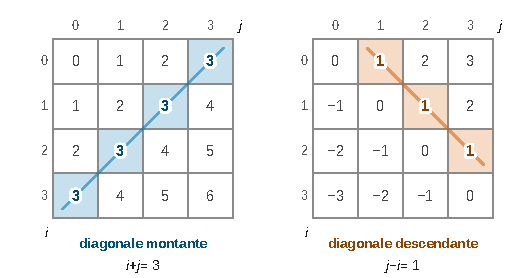
\includegraphics{figures/q07-invariants-diagonales.pdf}
\caption*{Figure 1 --- Valeurs de i + j et de j − i sur la grille 4 × 4 :
constantes le long d'une diagonale montante et d'une diagonale
descendante}
\end{figure}

Avec (d) (exactement \(n\) reines), ces conditions expriment que deux reines ne se contrôlent jamais.

\hypertarget{q8}{%
\subsubsection{Q8}\label{q8}}

\begin{lstlisting}[language=Python]
def tous_distincts(L):
    """True si les éléments de L sont deux à deux distincts, False sinon."""
    presents = dict()
    for x in L:
        if x in presents:       # x déjà rencontré : doublon
            return False
        presents[x] = True
    return True                 # parcours complet sans doublon
\end{lstlisting}

Invariant : au début de chaque tour, les clés de \texttt{presents} sont exactement les éléments déjà parcourus, et ceux-ci sont deux à deux distincts. Le \texttt{return\ True} final est donc correct. Chaque tour coûte \(O(1)\) (test d'appartenance et insertion dans un dictionnaire, annexe 2) : la fonction est en \(O(n)\) pour \(n = \texttt{len(L)}\).

\hypertarget{q9}{%
\subsubsection{Q9}\label{q9}}

Le code de l'étudiant comporte trois erreurs :

\begin{itemize}
\tightlist
\item
  ligne 3 : \texttt{range(i,\ n)} autorise \(j = i\), et le test \texttt{L{[}i{]}\ ==\ L{[}i{]}} est toujours vrai ; il faut \texttt{range(i+1,\ n)} ;
\item
  ligne 5 : deux éléments égaux signifient « pas tous distincts », il faut \texttt{return\ False} ;
\item
  ligne 6 : sans doublon, il faut \texttt{return\ True}.
\end{itemize}

En l'état, la fonction renvoie \texttt{True} pour toute liste non vide et \texttt{False} pour la liste vide.

\begin{lstlisting}[language=Python]
def tous_distincts2(L):
    n = len(L)
    for i in range(n):
        for j in range(i+1, n):
            if L[i] == L[j]:
                return False
    return True
\end{lstlisting}

\textbf{Complexités dans le pire des cas} (liste sans doublon, donc sans sortie anticipée) :

\begin{itemize}
\tightlist
\item
  \texttt{tous\_distincts} : \(n\) tours, chacun formé d'un test \texttt{x\ in\ presents} et d'une insertion, en \(O(1)\) d'après l'annexe 2, soit \(O(n)\) ;
\item
  \texttt{tous\_distincts2} : le nombre de comparaisons est \(\displaystyle\sum_{i=0}^{n-1}(n-1-i) = \frac{n(n-1)}{2}\), chacune en \(O(1)\), soit \(O(n^2)\).
\end{itemize}

\equationajustee{\boxed{\begin{aligned}{}&\texttt{tous\_distincts} : O(n) \\
&\texttt{tous\_distincts2} : O(n^2)
\end{aligned}}}

\hypertarget{q10}{%
\subsubsection{Q10}\label{q10}}

\begin{lstlisting}[language=Python]
def est_possible(L):
    """True si L vérifie les conditions (a), (b) et (c)."""
    sommes = []
    differences = []
    for i in range(len(L)):
        sommes.append(L[i] + i)
        differences.append(L[i] - i)
    return (tous_distincts(L) and tous_distincts(sommes)
            and tous_distincts(differences))
\end{lstlisting}

Le coût est en \(O(n)\). La fonction accepte des listes de longueur quelconque (elle servira en I.7 sur des configurations partielles).

\texttt{est\_possible(\allowbreak{}{[}2,\allowbreak{}\ 4,\allowbreak{}\ 1,\allowbreak{}\ 7,\allowbreak{}\ 0,\allowbreak{}\ 6,\allowbreak{}\ 3,\allowbreak{}\ 5{]}\allowbreak{})\allowbreak{}} renvoie \texttt{True} ; pour \texttt{{[}3,\allowbreak{}\ 4,\allowbreak{}\ 1,\allowbreak{}\ 7,\allowbreak{}\ 0,\allowbreak{}\ 6,\allowbreak{}\ 2,\allowbreak{}\ 5{]}\allowbreak{}}, les sommes \(3, 5, 3, 10, 4, 11, 8, 12\) contiennent deux fois \(3\) : la fonction renvoie \texttt{False}.

\hypertarget{q11}{%
\subsubsection{Q11}\label{q11}}

\begin{lstlisting}[language=Python]
def est_solution(L, n):
    """True si L vérifie (a), (b), (c) et (d)."""
    return len(L) == n and est_possible(L)
\end{lstlisting}

\texttt{est\_solution(\allowbreak{}{[}2,\allowbreak{}\ 0,\allowbreak{}\ 3,\allowbreak{}\ 1{]}\allowbreak{},\allowbreak{}\ 4)\allowbreak{}} renvoie \texttt{True}, \texttt{est\_solution(\allowbreak{}{[}0,\allowbreak{}\ 2,\allowbreak{}\ 3,\allowbreak{}\ 1{]}\allowbreak{},\allowbreak{}\ 4)\allowbreak{}} renvoie \texttt{False}.

\hypertarget{i.4-une-premiuxe8re-approche-par-recherche-aluxe9atoire}{%
\subsection{I.4 --- Une première approche par recherche aléatoire}\label{i.4-une-premiuxe8re-approche-par-recherche-aluxe9atoire}}

\hypertarget{q12}{%
\subsubsection{Q12}\label{q12}}

Les trois cadres du DR, avec l'appel imposé :

\begin{lstlisting}[language=Python]
# Méthode 1
import random as rd
rd.sample(L, len(L))

# Méthode 2
from random import sample
sample(L, len(L))

# Méthode 3
import random
random.sample(L, len(L))
\end{lstlisting}

La suite du sujet utilise la méthode 2 : \texttt{sample} s'appelle sans préfixe.

\hypertarget{q13}{%
\subsubsection{Q13}\label{q13}}

\begin{lstlisting}[language=Python]
from random import sample

def recherche_aleatoire(n, N):
    """Au plus N tirages de permutations de [0, ..., n-1] ;
    renvoie la première solution trouvée, ou [] en cas d'échec."""
    L = [i for i in range(n)]
    for essai in range(N):
        P = sample(L, len(L))       # permutation aléatoire de L
        if est_solution(P, n):
            return P                # arrêt dès qu'une solution est trouvée
    return []
\end{lstlisting}

Chaque permutation vérifie d'office (a) et (d) ; seules les diagonales sont réellement testées. Coût dans le pire des cas : \(O(nN)\).

\hypertarget{i.5-duxe9terminer-toutes-les-permutations-de-l-0-1-n-1}{%
\subsection{I.5 --- Déterminer toutes les permutations de L = {[}0, 1, \ldots, n-1{]}}\label{i.5-duxe9terminer-toutes-les-permutations-de-l-0-1-n-1}}

\hypertarget{q14}{%
\subsubsection{Q14}\label{q14}}

\begin{lstlisting}[language=Python]
def insertion(x, L, i):
    """Nouvelle liste : L avec x inséré à l'indice i (0 <= i <= len(L))."""
    M = []
    for k in range(i):              # termes d'indices 0 à i-1
        M.append(L[k])
    M.append(x)                     # x à la position i
    for k in range(i, len(L)):      # termes d'indices i à len(L)-1
        M.append(L[k])
    return M
\end{lstlisting}

\texttt{L} n'est pas modifiée. \texttt{insertion(\allowbreak{}5,\allowbreak{}\ {[}2,\allowbreak{}\ 3,\allowbreak{}\ 6,\allowbreak{}\ 4{]}\allowbreak{},\allowbreak{}\ 1)\allowbreak{}} donne \texttt{{[}2,\ 5,\ 3,\ 6,\ 4{]}} et \texttt{insertion(\allowbreak{}5,\allowbreak{}\ {[}2,\allowbreak{}\ 3,\allowbreak{}\ 6,\allowbreak{}\ 4{]}\allowbreak{},\allowbreak{}\ 4)\allowbreak{}} donne \texttt{{[}2,\ 3,\ 6,\ 4,\ 5{]}}.

\hypertarget{q15}{%
\subsubsection{Q15}\label{q15}}

À l'issue du premier passage dans la boucle externe (\texttt{l1\ =\ {[}0,\ 1{]}}), \(2\) a été inséré aux positions \(0, 1, 2\) :

\equationajustee{\boxed{P = [[2, 0, 1], [0, 2, 1], [0, 1, 2]]}}

Après l'exécution complète (second passage avec \texttt{l1\ =\ {[}1,\ 0{]}}) :

\equationajustee{\boxed{P = [[2, 0, 1], [0, 2, 1], [0, 1, 2], [2, 1, 0], [1, 2, 0], [1, 0, 2]]}}

\textbf{Ce code part des deux permutations de \(\{0, 1\}\) et insère la nouvelle valeur \(v = 2\) à chacune des \(v + 1 = 3\) positions possibles.}

\textbf{Il produit ainsi toutes les permutations de \(\{0, 1, 2\}\), chacune une seule fois.} Elles sont au nombre de

\equationajustee{\begin{aligned}
2 \times 3 &= 6 \\
&= 3!
\end{aligned}}

Une permutation de \(\{0, 1, 2\}\) est en effet déterminée par la position où figure \(2\), et par la permutation de \(\{0, 1\}\) qui reste quand on le retire.

\begin{figure}[H]
\centering
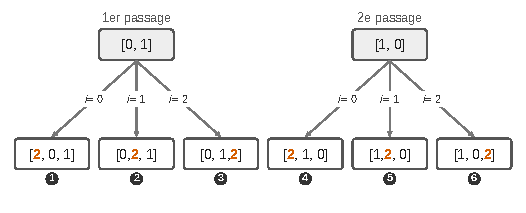
\includegraphics{figures/q15-arbre-insertions.pdf}
\caption*{Figure 2 --- Code de Q15 : chaque permutation de \{0, 1\} donne trois
permutations de \{0, 1, 2\} par insertion de 2 à la position i,
numérotées dans l'ordre des append}
\end{figure}

\hypertarget{q16}{%
\subsubsection{Q16}\label{q16}}

Squelette du DR complété : à chaque tour, \texttt{L} contient les permutations de \(\{0, \dots, v-1\}\) et on construit dans \texttt{P} celles de \(\{0, \dots, v\}\), comme en Q15.

\begin{lstlisting}[language=Python]
def permutations(n) :
    L = [[0]]
    for v in range(1, n) :
        P = []
        for l1 in L :
            for i in range(v+1) :
                P.append(insertion(v, l1, i))
        L = P
    return L
\end{lstlisting}

Invariant : au début du tour d'indice \(v\), \texttt{L} contient exactement une fois chaque permutation de \(\{0, \dots, v-1\}\). C'est vrai pour \(v = 1\) avec \texttt{{[}{[}0{]}{]}}.

Soit \(\sigma\) une permutation de \(\{0, \dots, v\}\). Notons \(i\) la position de \(v\) dans \(\sigma\).

Retirer cette valeur donne une liste \(s\), qui est une permutation de \(\{0, \dots, v-1\}\).

Alors \(\sigma\) s'écrit \texttt{insertion(\allowbreak{}v,\allowbreak{}\ s,\allowbreak{}\ i)\allowbreak{}}, et ce couple \texttt{(s,\ i)} est le seul qui convienne. Donc \texttt{P} contient chaque permutation de \(\{0, \dots, v\}\) exactement une fois.

À la fin, \texttt{L} contient les \(n!\) permutations de \(\{0, \dots, n-1\}\). On ne construit pas la nouvelle génération dans la liste en cours de parcours : d'où la liste auxiliaire \texttt{P}.

\texttt{permutations(3)} renvoie \texttt{{[}{[}2,\allowbreak{}\ 1,\allowbreak{}\ 0{]}\allowbreak{},\allowbreak{}\ {[}1,\allowbreak{}\ 2,\allowbreak{}\ 0{]}\allowbreak{},\allowbreak{}\ {[}1,\allowbreak{}\ 0,\allowbreak{}\ 2{]}\allowbreak{},\allowbreak{}\ {[}2,\allowbreak{}\ 0,\allowbreak{}\ 1{]}\allowbreak{},\allowbreak{}\ {[}0,\allowbreak{}\ 2,\allowbreak{}\ 1{]}\allowbreak{},\allowbreak{}\ {[}0,\allowbreak{}\ 1,\allowbreak{}\ 2{]}\allowbreak{}{]}\allowbreak{}}.

\hypertarget{q17}{%
\subsubsection{Q17}\label{q17}}

\begin{lstlisting}[language=Python]
def configurations(n):
    """Liste de toutes les solutions du problème des n reines."""
    C = []
    for p in permutations(n):
        if est_solution(p, n):
            C.append(p)
    return C
\end{lstlisting}

Toute solution est une permutation de \(\{0, \dots, n-1\}\), d'après (a) et (d) : le filtrage n'en perd aucune.

On retrouve \texttt{len(\allowbreak{}configurations(\allowbreak{}5)\allowbreak{})\allowbreak{}\ =\allowbreak{}=\allowbreak{}\ 10} et \texttt{len(\allowbreak{}configurations(\allowbreak{}8)\allowbreak{})\allowbreak{}\ =\allowbreak{}=\allowbreak{}\ 92}. Coût : \(n!\) tests en \(O(n)\), soit \(O(n \cdot n!)\).

\hypertarget{i.6-classer-les-configurations-similaires}{%
\subsection{I.6 --- Classer les configurations similaires}\label{i.6-classer-les-configurations-similaires}}

\hypertarget{q18}{%
\subsubsection{Q18}\label{q18}}

Lecture de la figure 6, à partir de \(L = [2, 4, 1, 3, 0]\) :

\equationajustee{\boxed{\begin{aligned}
L1 &= [0, 3, 1, 4, 2] \\
L2 &= [0, 2, 4, 1, 3]
\end{aligned}}}

La symétrie horizontale (d'axe horizontal) échange les lignes \(i\) et \(n - 1 - i\) sans changer les colonnes. La reine \((i, L[i])\) va donc en \((n-1-i, L[i])\), d'où

\equationajustee{\boxed{L1[i] = L[n-1-i] \text{ pour tout } i}}

\textbf{La liste de la symétrie horizontale est la liste \(L\) lue à l'envers.} Contrôle : \([2, 4, 1, 3, 0]\) renversée donne \([0, 3, 1, 4, 2]\). De même, la règle de Q20 appliquée à \(L\) redonne \(L2\).

\hypertarget{q19}{%
\subsubsection{Q19}\label{q19}}

\begin{lstlisting}[language=Python]
def symetrie(L):
    """Configuration obtenue par symétrie d'axe horizontal."""
    n = len(L)
    M = []
    for i in range(n):
        M.append(L[n-1-i])      # indices n-1, n-2, ..., 0
    return M
\end{lstlisting}

\texttt{symetrie(\allowbreak{}{[}1,\allowbreak{}\ 0,\allowbreak{}\ 2{]}\allowbreak{})\allowbreak{}} renvoie \texttt{{[}2,\ 0,\ 1{]}}. Coût \(O(n)\) ; aucun indice négatif ni outil interdit.

\hypertarget{q20}{%
\subsubsection{Q20}\label{q20}}

La reine \((i, L[i])\) arrive en ligne \(L[i]\), colonne \(n - 1 - i\). La liste image \(M\) vérifie donc

\equationajustee{M[L[i]] = n - 1 - i.}

Les lignes d'arrivée ne sont pas produites dans l'ordre, donc on crée d'abord une liste de taille \(n\) et on remplit chaque case à sa place.

\begin{lstlisting}[language=Python]
def rotation(L):
    """Configuration obtenue par rotation d'un quart de tour vers la droite."""
    n = len(L)
    M = ligne(n)                # liste de n zéros
    for i in range(n):
        M[L[i]] = n - 1 - i
    return M
\end{lstlisting}

Comme \(L\) est une permutation de \(\{0, \dots, n-1\}\), chaque case de \(M\) est écrite exactement une fois.

\texttt{rotation(\allowbreak{}{[}2,\allowbreak{}\ 5,\allowbreak{}\ 3,\allowbreak{}\ 1,\allowbreak{}\ 7,\allowbreak{}\ 4,\allowbreak{}\ 6,\allowbreak{}\ 0{]}\allowbreak{})\allowbreak{}} renvoie \texttt{{[}0,\allowbreak{}\ 4,\allowbreak{}\ 7,\allowbreak{}\ 5,\allowbreak{}\ 2,\allowbreak{}\ 6,\allowbreak{}\ 1,\allowbreak{}\ 3{]}\allowbreak{}}. Par exemple, \(L[7] = 0\) donne

\equationajustee{\begin{aligned}
M[0] &= 8 - 1 - 7 \\
&= 0.
\end{aligned}}

\hypertarget{q21}{%
\subsubsection{Q21}\label{q21}}

\textbf{Ligne 1.} \texttt{C\ =\allowbreak{}\ configurations(\allowbreak{}n)\allowbreak{}} calcule (fonction de Q17) la liste de toutes les solutions du problème des \(n\) reines, que la fonction va classer.

\textbf{Type.} \texttt{partition(n)} renvoie une \textbf{liste}.

\textbf{Structure.} C'est une liste de listes de listes d'entiers :

\begin{itemize}
\tightlist
\item
  chaque élément \texttt{elt} de \texttt{P} est une \textbf{classe} : une liste non vide de configurations deux à deux similaires ;
\item
  chaque configuration est une liste de \(n\) entiers de \(\{0, \dots, n-1\}\) ;
\item
  \texttt{elt{[}0{]}}, la première configuration rencontrée de la classe, en est le représentant ;
\item
  les classes sont disjointes et leur réunion est l'ensemble des solutions : \texttt{P} est une partition de \texttt{C}.
\end{itemize}

\textbf{Fonctionnement.} La fonction parcourt les solutions une à une. Pour chaque solution \texttt{c}, elle compare \texttt{c} au représentant \texttt{elt{[}0{]}} de chaque classe déjà formée. Si \texttt{c} est similaire à l'un d'eux, \texttt{c} est ajoutée à cette classe et \texttt{test} passe à \texttt{True}. Si, après examen de toutes les classes, \texttt{test} vaut encore \texttt{False}, \texttt{c} n'est similaire à aucune et fonde une nouvelle classe \texttt{{[}c{]}}. La similarité étant une relation d'équivalence, comparer au seul représentant suffit, et \texttt{c} ne peut être similaire qu'à un seul représentant. Par exemple, pour \(n = 5\) on obtient deux classes, de 8 et de 2 configurations.

\hypertarget{i.7-des-graphes-pour-aller-plus-vite-et-plus-loin}{%
\subsection{I.7 --- Des graphes pour aller plus vite et plus loin}\label{i.7-des-graphes-pour-aller-plus-vite-et-plus-loin}}

\hypertarget{q22}{%
\subsubsection{Q22}\label{q22}}

Squelette du DR complété. Un sommet du graphe est une configuration partielle \texttt{L} (reines des lignes \(0\) à \texttt{len(L)\ -\ 1}) ; ses fils sont les \texttt{L\ +\ {[}i{]}}.

\begin{lstlisting}[language=Python]
def explore(L, n):
    if not est_possible(L):
        return -1                  # grille invalide : on revient en arrière
    if len(L) == n:                 # si fin de recherche victorieuse
        return L
    for i in range(n):
        res = explore(L + [i], n)
        if res != -1:              # si une solution a été trouvée
            return res
    return -1                       # aucun fils ne mène à une solution

def resout_graphe(n):
    rep = explore([], n)
    return rep
\end{lstlisting}

Le test de validité vient avant le test de longueur : une liste de longueur \(n\) n'est renvoyée que si elle vérifie (a), (b), (c), donc elle vérifie aussi (d) et c'est une solution. Une configuration invalide n'est jamais prolongée (aucune solution ne peut prolonger une configuration où deux reines se contrôlent) : c'est l'élagage qui évite de visiter tout le graphe. Le \texttt{return\ res} arrête le parcours dès la première solution ; le dernier \texttt{return\ -1} signale l'échec à l'appelant, qui essaie la colonne suivante. La fonction termine car \(n - \texttt{len(L)}\) décroît strictement à chaque appel récursif. On obtient \texttt{resout\_graphe(\allowbreak{}4)\allowbreak{}\ =\allowbreak{}=\allowbreak{}\ {[}1,\allowbreak{}\ 3,\allowbreak{}\ 0,\allowbreak{}\ 2{]}\allowbreak{}} et \texttt{resout\_graphe(\allowbreak{}8)\allowbreak{}\ =\allowbreak{}=\allowbreak{}\ {[}0,\allowbreak{}\ 4,\allowbreak{}\ 7,\allowbreak{}\ 5,\allowbreak{}\ 2,\allowbreak{}\ 6,\allowbreak{}\ 1,\allowbreak{}\ 3{]}\allowbreak{}}.

\begin{figure}[H]
\centering
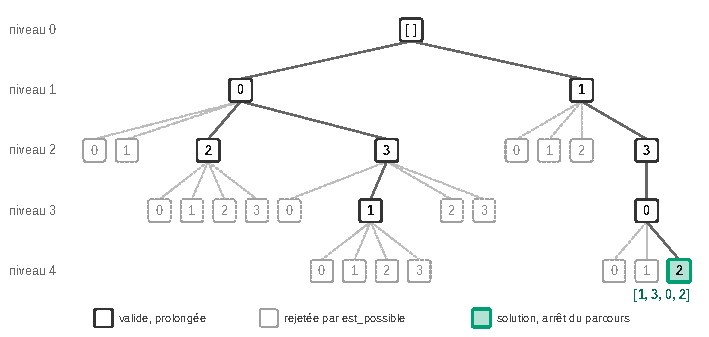
\includegraphics{figures/q22-arbre-retour-sur-trace.pdf}
\caption*{Figure 3 --- Sommets visités par resout\_graphe(4) : une configuration
rejetée par est\_possible n'est pas prolongée, et le parcours s'arrête à
la première solution}
\end{figure}

\hypertarget{q23}{%
\subsubsection{Q23}\label{q23}}

Squelette du DR complété : chaque appel renvoie le \textbf{nombre} de solutions qui prolongent \texttt{L}, et le parcours ne s'arrête plus à la première.

\begin{lstlisting}[language=Python]
def explore2(L, n):
    if not est_possible(L):
        return 0                           # aucune solution ne prolonge L
    if len(L) == n:
        return 1                           # L est une solution
    nb_sol = 0
    for i in range(n):
        nb_sol = nb_sol + explore2(L + [i], n)
    return nb_sol

def compte(n):
    rep = explore2([], n)
    return rep
\end{lstlisting}

Les solutions qui prolongent une configuration partielle valide \texttt{L} (de longueur \(< n\)) se répartissent, sans recouvrement, selon la colonne \texttt{i} de la reine de la ligne \texttt{len(L)} : leur nombre est la somme des nombres de solutions prolongeant les \texttt{L\ +\ {[}i{]}}. Par récurrence sur \(n - \texttt{len(L)}\), \texttt{explore2(L,\ n)} renvoie donc le nombre de solutions prolongeant \texttt{L}. On retrouve \texttt{compte(4)\ ==\ 2}, \texttt{compte(5)\ ==\ 10}, \texttt{compte(6)\ ==\ 4} et \texttt{compte(8)\ ==\ 92}.

\hypertarget{partie-ii-base-de-donnuxe9es-dun-serveur-de-jeu-en-ligne}{%
\section{Partie II --- Base de données d'un serveur de jeu en ligne}\label{partie-ii-base-de-donnuxe9es-dun-serveur-de-jeu-en-ligne}}

\hypertarget{q24}{%
\subsubsection{Q24}\label{q24}}

L'attribut \texttt{anniversaire} est au format \texttt{\textquotesingle{}JJ-MM\textquotesingle{}} : le 3 juillet s'écrit \texttt{\textquotesingle{}03-07\textquotesingle{}}.

\begin{lstlisting}[language=SQL]
SELECT nom, prenom, email
FROM Clients
WHERE anniversaire = '03-07';
\end{lstlisting}

\hypertarget{q25}{%
\subsubsection{Q25}\label{q25}}

\begin{figure}[H]
\centering
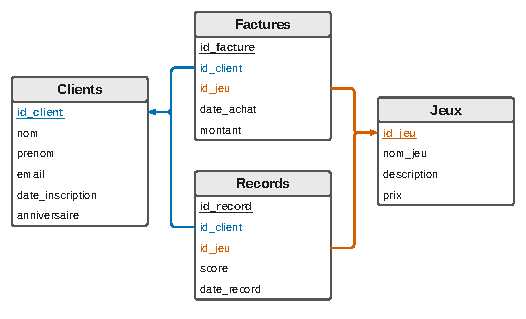
\includegraphics{figures/q25-schema-relationnel.pdf}
\caption*{Figure 4 --- Schéma de la base : clés primaires soulignées, clés
étrangères de Factures et Records vers Clients et Jeux}
\end{figure}

Le nom et le prénom sont dans \texttt{Clients}, les dates d'achat dans \texttt{Factures} : jointure sur \texttt{id\_client}.

\begin{lstlisting}[language=SQL]
SELECT Clients.nom, Clients.prenom, Factures.date_achat
FROM Clients
JOIN Factures ON Clients.id_client = Factures.id_client
WHERE Clients.email = 'myriam.sarr@ccinp.edu';
\end{lstlisting}

Une ligne est renvoyée par achat de ce client.

\hypertarget{q26}{%
\subsubsection{Q26}\label{q26}}

On regroupe les factures par client (sur la clé primaire, pour ne pas fusionner deux homonymes) et on somme les montants.

\begin{lstlisting}[language=SQL]
SELECT Clients.nom, Clients.email, SUM(Factures.montant) AS total
FROM Clients
JOIN Factures ON Clients.id_client = Factures.id_client
GROUP BY Clients.id_client, Clients.nom, Clients.email;
\end{lstlisting}

Avec cette jointure interne, un client qui n'a fait aucun achat n'apparaît pas dans le résultat (son total serait nul). On peut ajouter \texttt{ORDER\ BY\ total\ DESC} pour classer les meilleurs clients en tête.

\hypertarget{q27}{%
\subsubsection{Q27}\label{q27}}

\begin{lstlisting}[language=SQL]
SELECT Jeux.nom_jeu, MAX(Records.score) AS meilleur_score
FROM Jeux
JOIN Records ON Jeux.id_jeu = Records.id_jeu
GROUP BY Jeux.id_jeu, Jeux.nom_jeu;
\end{lstlisting}

On obtient une ligne par jeu ayant au moins un record, avec son meilleur score. Un \texttt{ORDER\ BY\ score\ DESC\ LIMIT\ 1} ne conviendrait pas : il donnerait le meilleur score tous jeux confondus.

\textbf{FIN}

\end{document}
